\subsection{Experimentación}

En esta parte del informe nos dedicaremos a corroborar empíricamente ciertas hipótesis sobre nuestra herística golosa.

Primero intentamos ver que la complejidad del peor caso, $\O(n_1^4.n_2)$ sea una cota superior correcta. Esto es corroborado en el siguiente gráfico.

\begin{figure}[H]
 \centering
	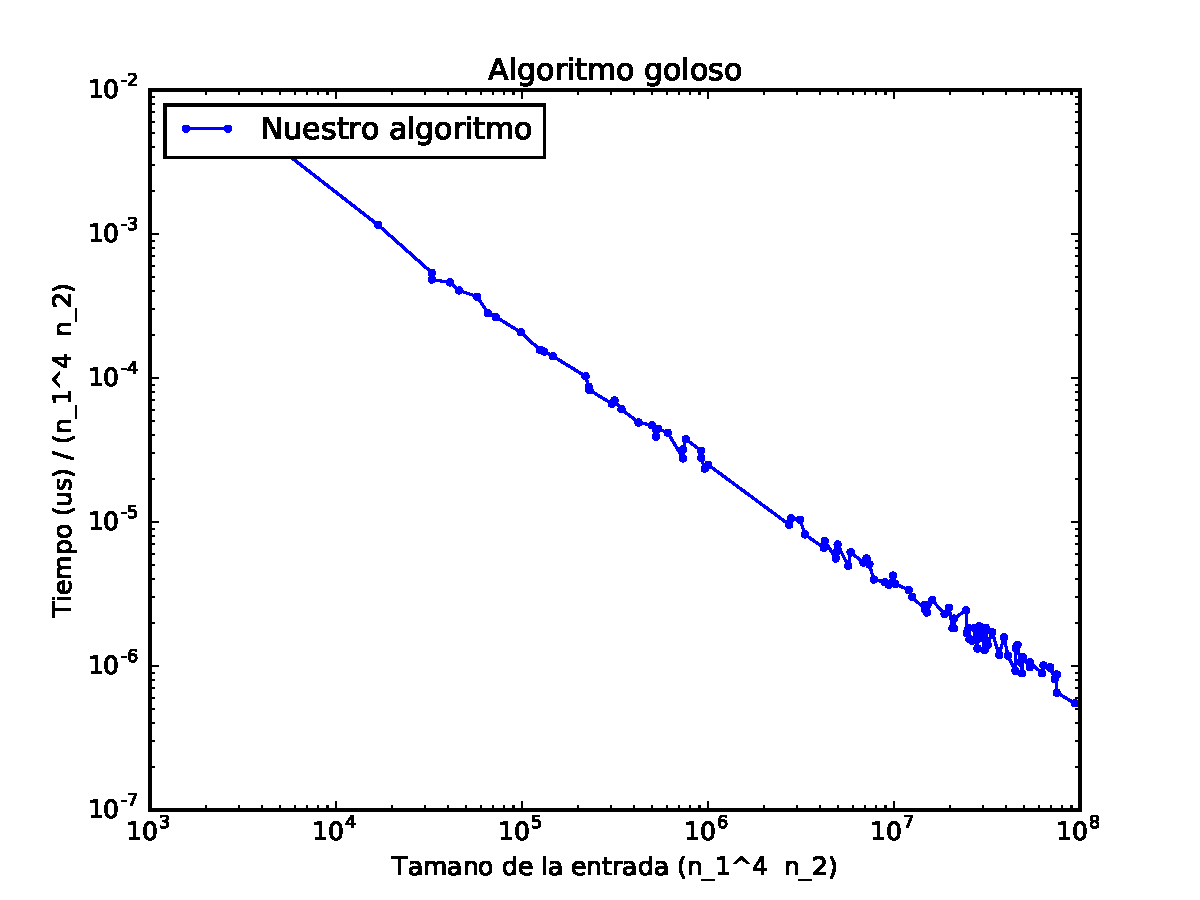
\includegraphics[width=0.9\textwidth]{graficos/problema_4/tiempos_1.pdf}
	\caption{}
	\label{fig:problema4-1}
\end{figure}

Se puede observar como, para instancias cada vez mas grandes, el tiempo en relación a la cota esperada decrece tendiendo a cero, de esto se puede deducir que nuestra cota no es la mas ajustada posible, o sea no serviría como cota inferior.

Como se puede observar, la complejidad que calculamos previamente depende de dos variables, $n_1$ y $n_2$, los siguientes gráficos analizan por separado que pasa cuando se varía cada uno de estos valores y se intenta corroborar que la complejidad es correcta.

\begin{figure}[H]
 \centering
	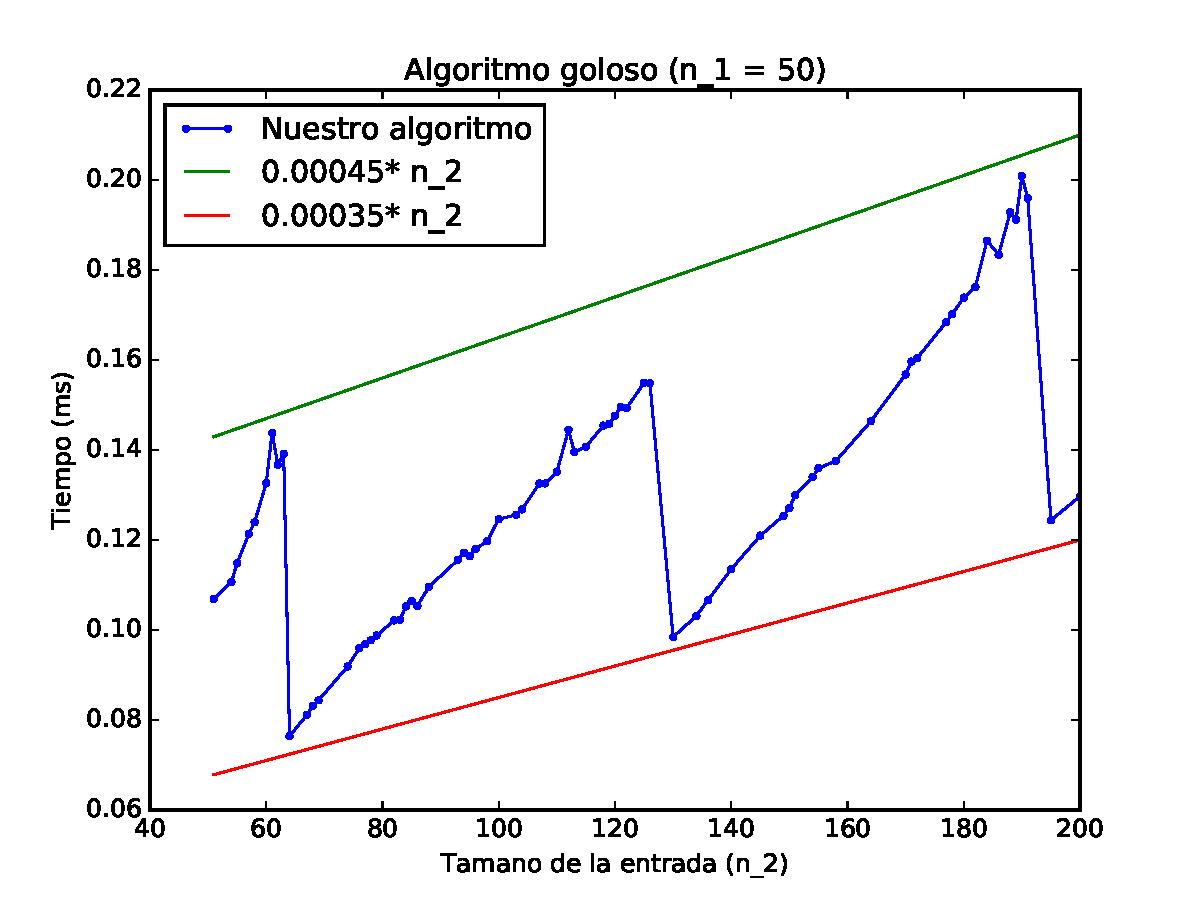
\includegraphics[width=0.9\textwidth]{graficos/problema_4/tiempos_2.pdf}
	\caption{}
	\label{fig:problema4-2}
\end{figure}

Este gráfico tiene dos particularidades que valen la pena comentar. Primero que púdimos ajustar el problema inferior y superiormente para esta variable. Segundo que hay picos, esto se debe a la manera en que maneja c++ a los vectores, estos se copian y aumentan de tamaño al pasar un tamaño multiplo de 64 elementos.

\begin{figure}[H]
 \centering
	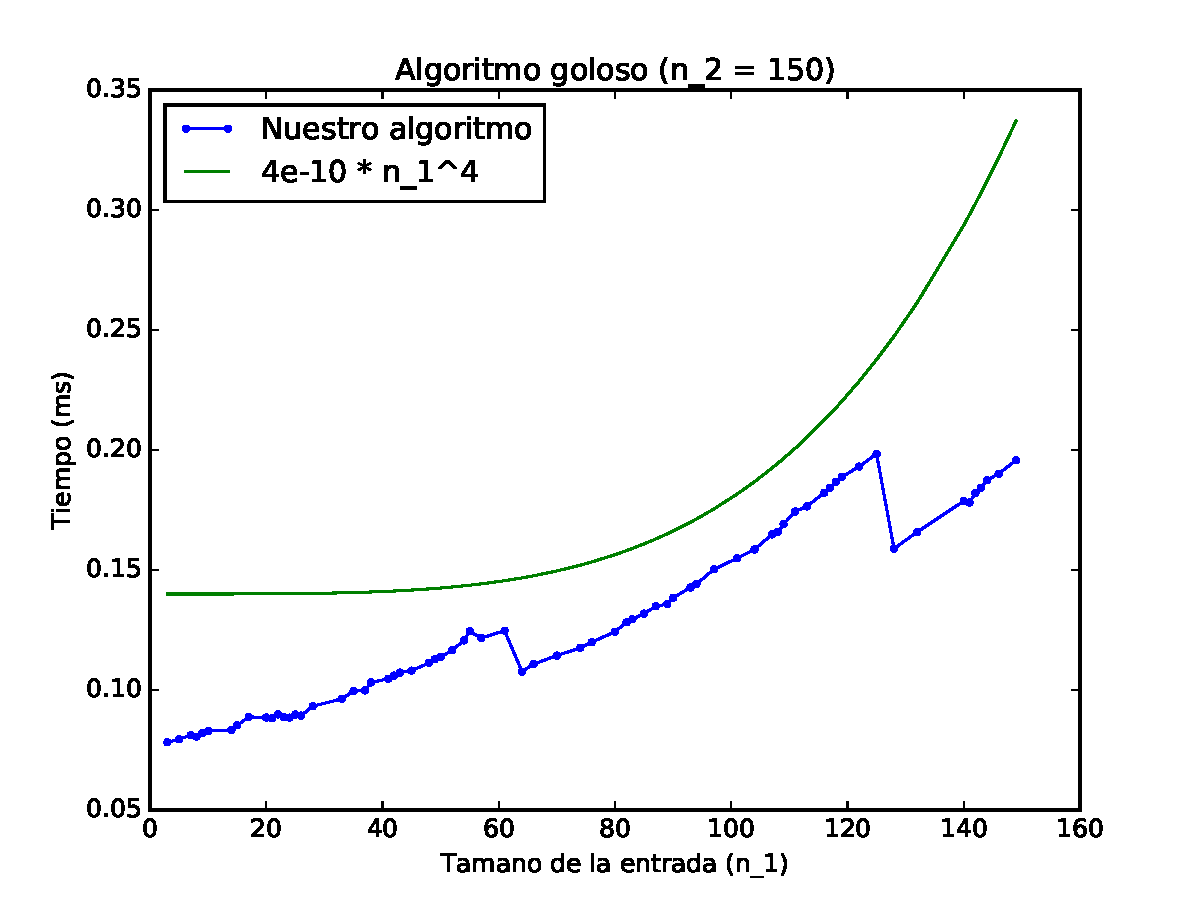
\includegraphics[width=0.9\textwidth]{graficos/problema_4/tiempos_3.pdf}
	\caption{}
	\label{fig:problema4-3}
\end{figure}

En este gráfico se ve como acotamos superiormente las instancias generadas con la complejidad que habiamos calculado y variando solo $n_1$.

La siguiente fígura expone la cantidad de aristas que tenian los isomorfismos calculados por nuestras dos heurísticas golosas, la mala (la primera) y la segunda, la que escogimos como nuestro algoritmo predilecto.

\begin{figure}[H]
 \centering
	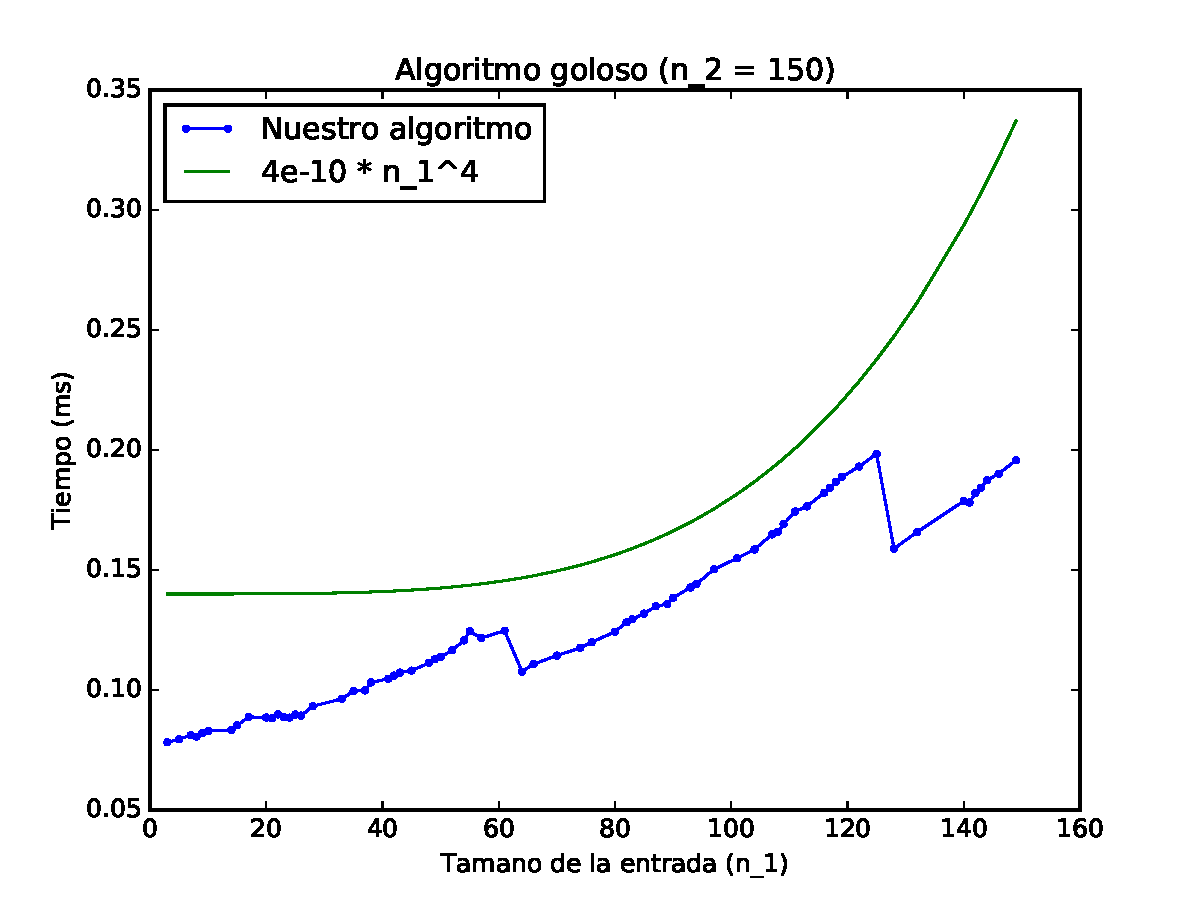
\includegraphics[width=0.9\textwidth]{graficos/problema_4/calidad.pdf}
	\caption{}
	\label{fig:problema4-4}
\end{figure}

Se puede ver como nuestro algoritmo siempre es en promedio superior. Aunque la ventaja no es tampoco inmensa, lo cual deja a criterio de la aplicación deseada si es preferible usar una u otra, ya que si recordamos lo dicho antes, la complejidad del Goloso Malo es bastante mejor, $O(n_2^2)$.

\subsection{Método de experimentación}